\documentclass{article}
\usepackage{polski}
\usepackage[utf8]{inputenc}
\usepackage[OT4]{fontenc}
\usepackage{graphicx,color}
\usepackage{url}
\usepackage[pdftex,hyperfootnotes=false,pdfborder={0 0 0}]{hyperref}
\usepackage{float}

\begin{document}
\thispagestyle{empty} %bez numeru strony

\begin{center}
{\large{Sprawozdanie z laboratorium:\\
Informatyka w Medycynie}}

\vspace{3ex}

Tomograf

\vspace{3ex}
{\footnotesize\today}

\end{center}


\vspace{10ex}

Prowadzący: Iwo Błądek

\vspace{5ex}

Autorzy:
\begin{tabular}{lllr}
\textbf{Adam Pioterek} & inf122446 & adam.pioterek@student.put.poznan.pl \\
\textbf{Marcin Drzewiecki} & inf122472 & marcin.drzewiecki@student.put.poznan.pl \\
\end{tabular}

\newpage



\section{Opis ćwiczenia}


\section{Algorytm}
\begin{description}
\item[1)] Wczytujemy obraz, konwertujemy do skali szarości.
\item[2)] Wybieramy liczbę emiterów, krok, liczbę receptorów przypadającą na jeden emiter, rozwartość kątową.
\item[3)] Dla każdej projekcji emiter-receptor za pomocą algorytmu Bresenhama wyznaczamy piksele należące do linii. Dla każdej linii wyznaczamy średnią wartość pikseli leżących na niej. W ten sposób uzyskujemy sinogram.
\item[4)] Na podstawie sinogramu odtwarzamy obraz: dla każdego elementu sinogramu (projekcji emiter-receptor) dodajemy do wartości piksela średnią wartość piksela odczytaną z tablicy. 
\item[5)] Wpisujemy wyniki do tablicy wynikowej reprezentującej obraz, normalizujemy wartości pikseli oraz stosujemy filtr uwzględniający gęstość linii przechodzących przez dany obszar obrazu[1]
\item[6)] Zapisujemy obraz oraz proces jego odtwarzania.
\end{description}
 
\section{Wynik działania programu}

\subsection{Przekształcenia}
\begin{figure}[H]
\begin{center}
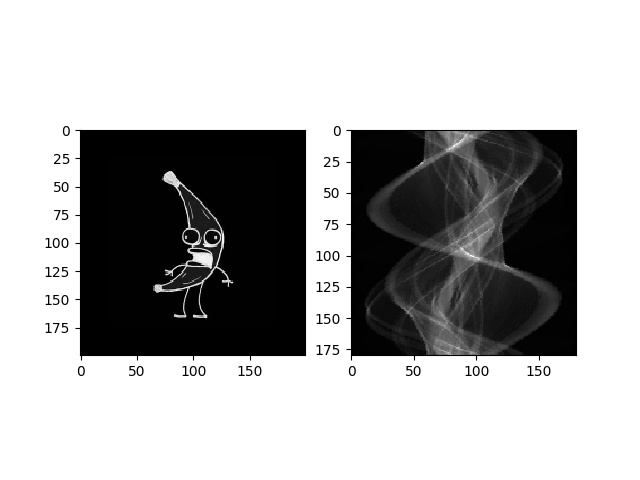
\includegraphics[width=0.8\textwidth]{./banana/sinogram.jpg}
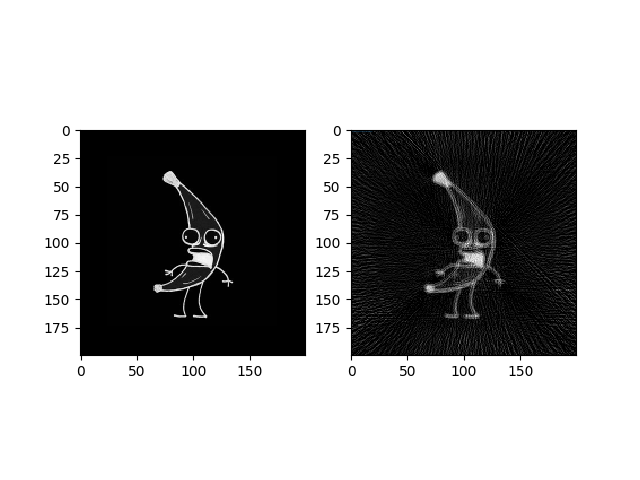
\includegraphics[width=0.8\textwidth]{./banana/reconstructedPicture2.png}
\end{center}
\end{figure}

\subsection{Przekształcenia}
\begin{figure}[H]
\begin{center}
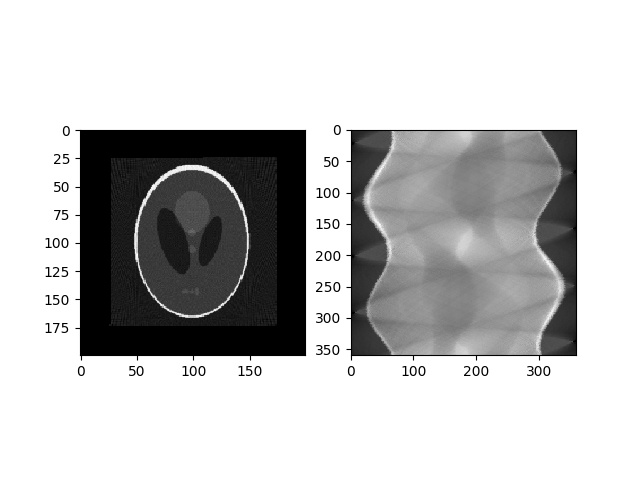
\includegraphics[width=0.8\textwidth]{./phantom/sinogram.jpg}
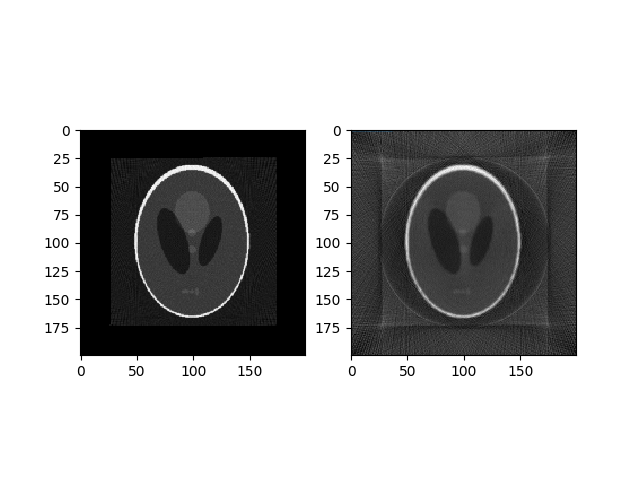
\includegraphics[width=0.8\textwidth]{./phantom/reconstructedImg2.png}
\end{center}
\end{figure}

\subsection{Przekształcenia}
\begin{figure}[H]
\begin{center}
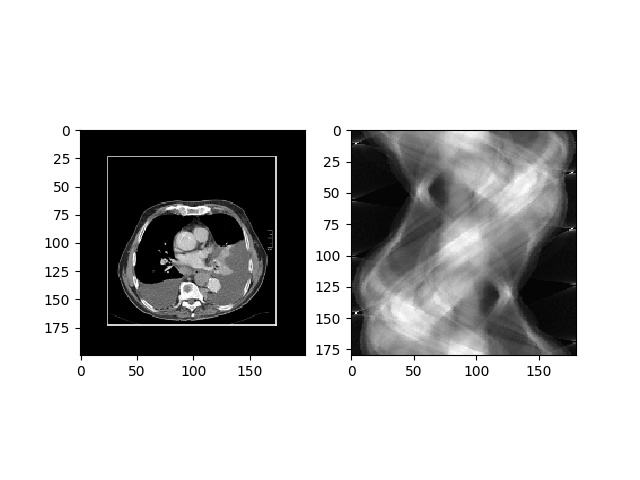
\includegraphics[width=0.8\textwidth]{./something/sinogram.jpg}
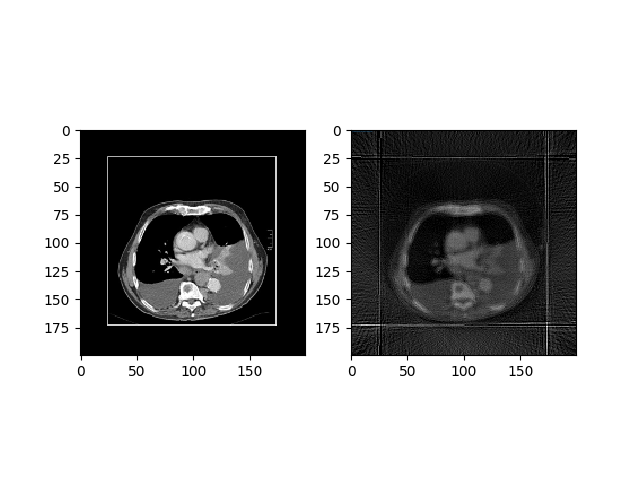
\includegraphics[width=0.8\textwidth]{./something/reconstructedImg2.png}
\end{center}
\end{figure}

\subsection{Przekształcenia}
\begin{figure}[H]
\begin{center}
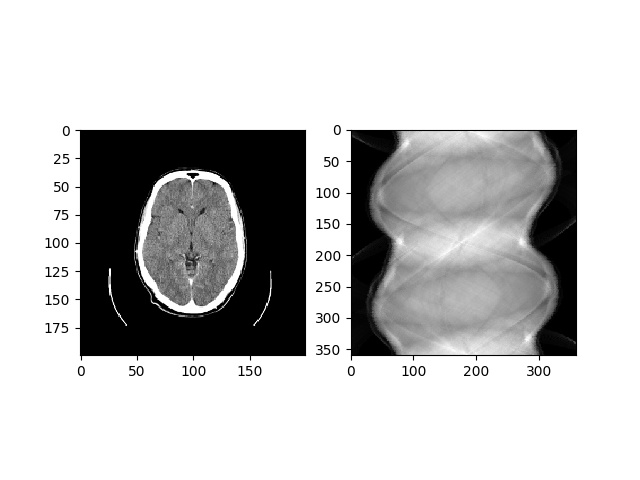
\includegraphics[width=0.8\textwidth]{./brain/sinogram.jpg}
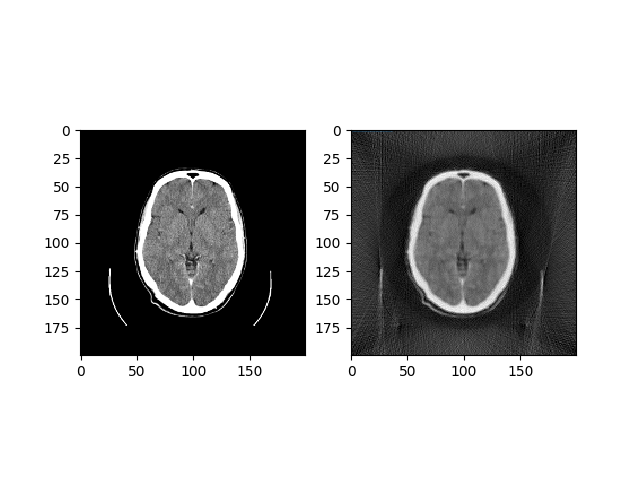
\includegraphics[width=0.8\textwidth]{./brain/reconstructedImg2.png}
\end{center}
\end{figure}


\section{Bibliografia}
[1]{http://www.dspguide.com/ch25/5.htm}

\end{document}
